% --- TabPFN and TRIBE v2 ---
% % --- Tabular Foundation Models: TabPFN ---
\begin{frame}{TabPFN: Prior-Data Fitted Network}
  \begin{itemize}
    \item Trained to ``meta-learn'' classification solutions for tabular datasets; pretraining uses millions of \textbf{synthetic} datasets, never real data.
    \item A new dataset is handled by \textbf{in-context learning}: the training rows go in as context, and predictions come out in one forward pass, in under a second.
    \item Zero-shot predictions for new, small tabular datasets.
    \item TabPFN v2 (published in \emph{Nature}, 2025) extends this to regression, missing values, and larger tables.
    \item Applications: Science data analysis, health records, finance.
  \end{itemize}
\end{frame}

\begin{frame}{TabPFN: Architecture and Capabilities}
  \centering
  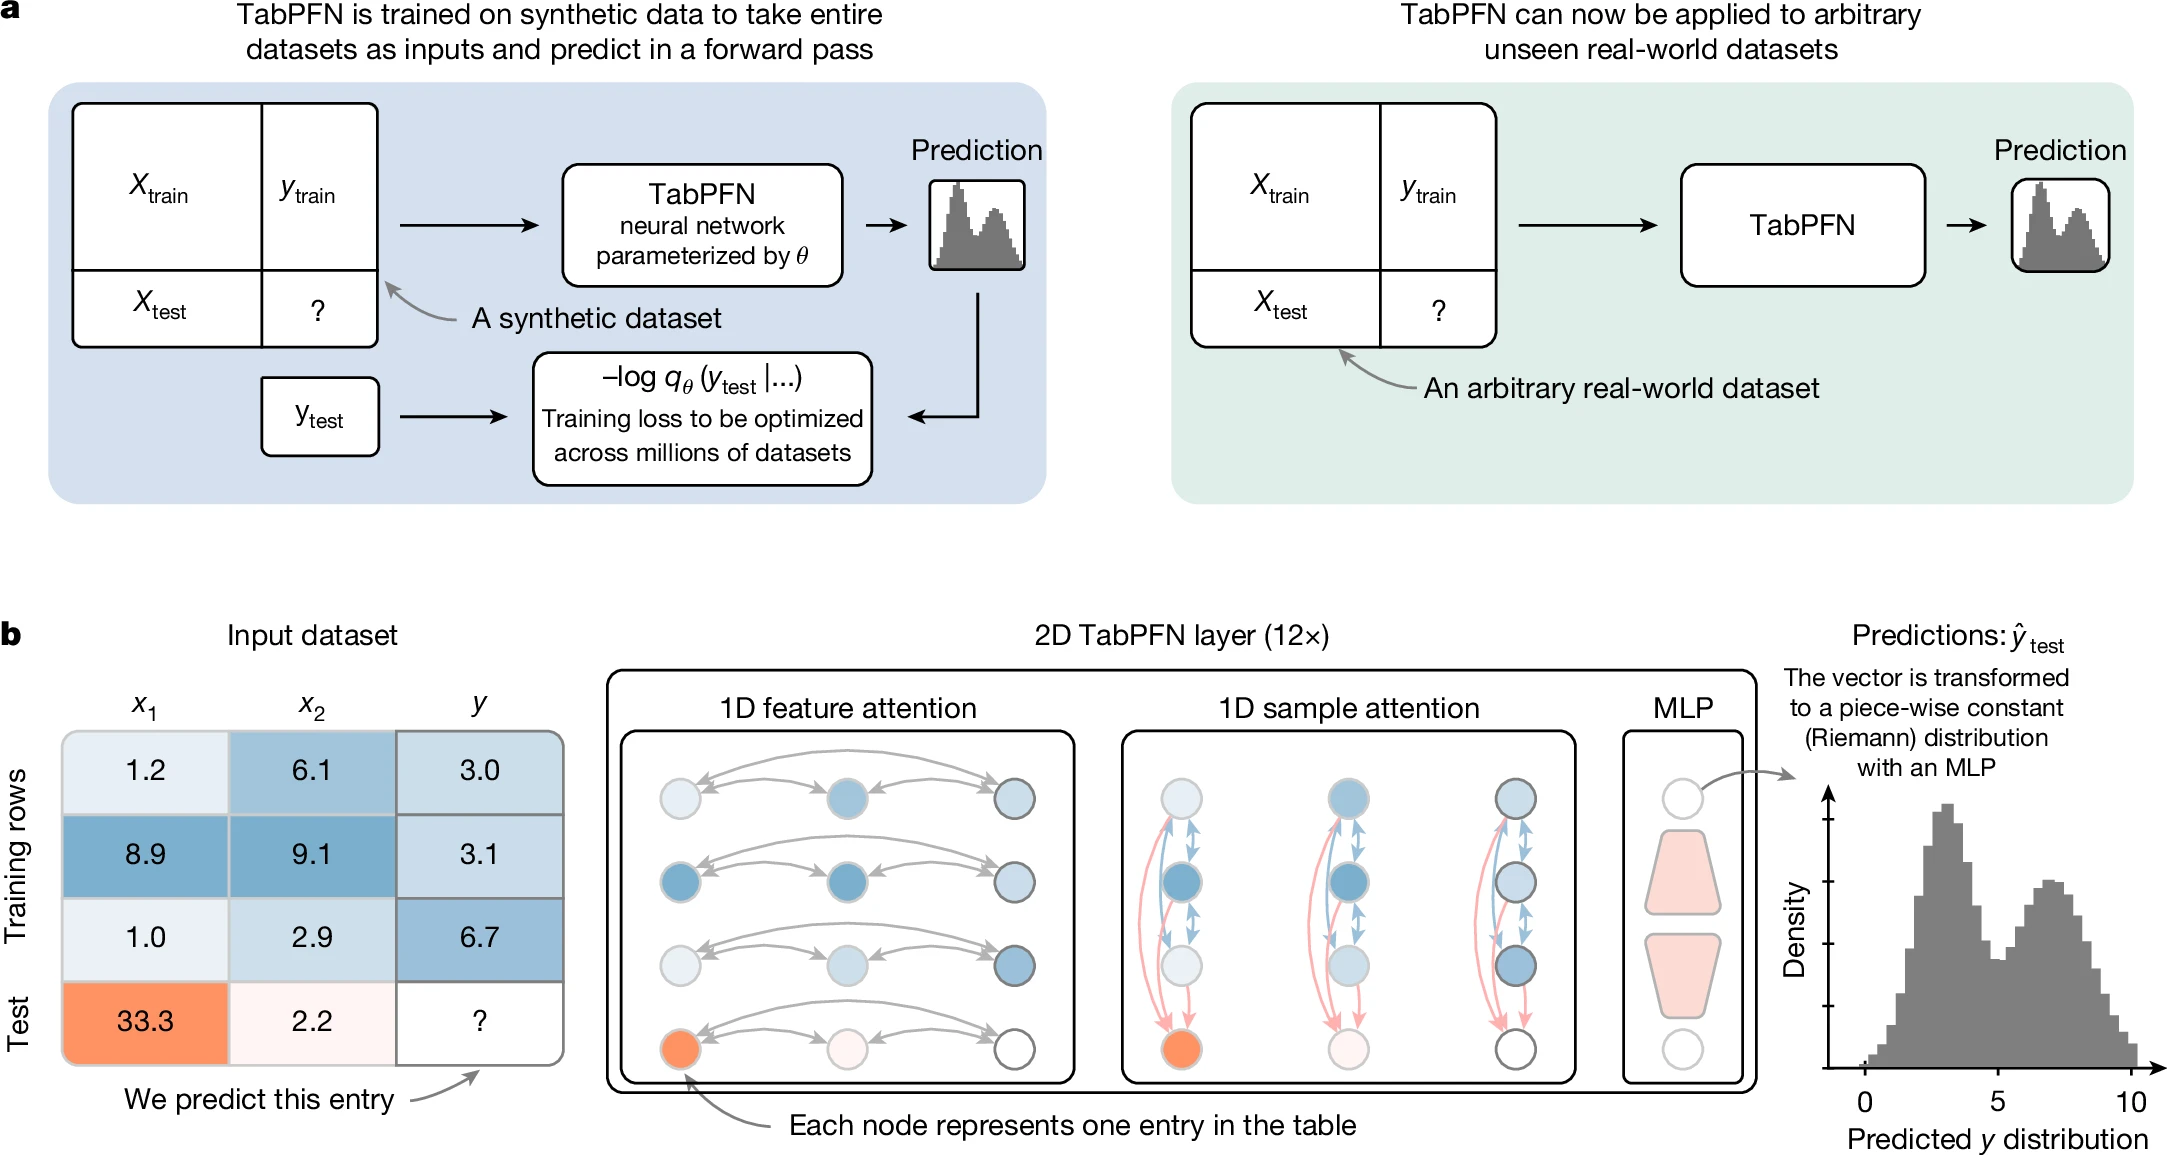
\includegraphics[width=0.85\textwidth, height=0.56\textheight, keepaspectratio]{images/foundation-models/tabpfn_summary.png}\\[0.15em]
  {\scriptsize Hollmann et al., ``TabPFN: A Transformer That Solves Small Tabular Classification Problems in a Second,'' ICLR 2023 (\href{https://arxiv.org/abs/2207.01848}{arXiv:2207.01848})}\\[0.15em]
  \begin{itemize}\footnotesize
    \item Learns a prior over tabular tasks by pretraining on large synthetic task distributions.
    \item Performs in-context learning on a new dataset in one forward pass.
    \item Two-way attention captures dependencies across both rows and features.
  \end{itemize}
\end{frame}

% --- Medical Foundation Models: Tribe v2 ---
\begin{frame}{Medical Foundation Models: TRIBE v2}
  \begin{columns}[T,onlytextwidth]
    \begin{column}{0.44\textwidth}
      \begin{itemize}
        \item Model of brain-response dynamics.
        \item Frozen encoders for video/audio/text + transformer integration backbone.
        \item Supports zero-shot transfer to unseen subjects/tasks at population level.
      \end{itemize}
    \end{column}
    \begin{column}{0.56\textwidth}
      \centering
      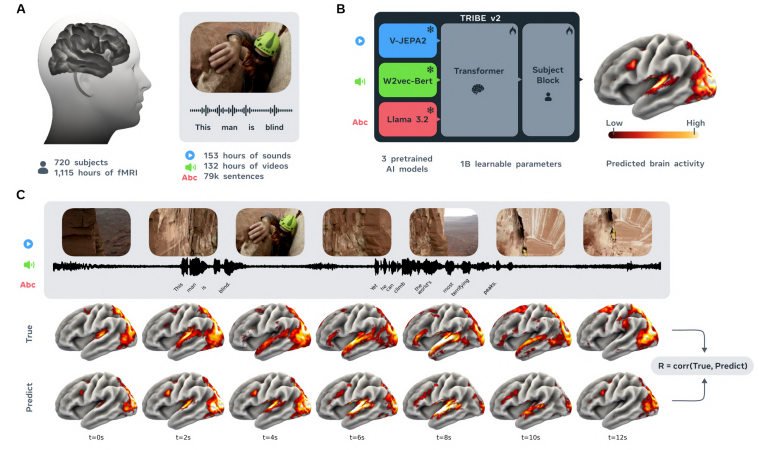
\includegraphics[width=\linewidth]{images/foundation-models/tribe_v2_arxiv_fig1_approach.png}\\[0.15em]
      {\scriptsize Figure from Meta AI's TRIBE v2 announcement: data $\rightarrow$ pretrained embeddings $\rightarrow$ predicted cortical response vs.\ measured mean response}
    \end{column}
  \end{columns}
\end{frame}

\begin{frame}{TRIBE v2: Encoding Performance (Results)}
  \begin{columns}[T,onlytextwidth]
    \begin{column}{0.48\textwidth}
      \centering
      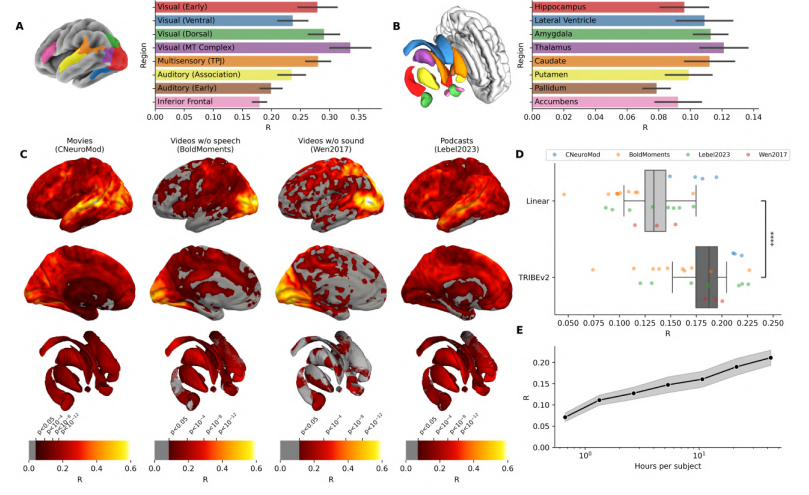
\includegraphics[width=\linewidth]{images/foundation-models/tribe_v2_arxiv_fig2_encoding_results.png}\\[0.15em]
      {\scriptsize Figure from Meta AI's TRIBE v2 announcement: Cortical/subcortical encoding scores; vs.\ linear baseline; scaling with training data.}
    \end{column}
    \begin{column}{0.48\textwidth}
      \begin{itemize}\footnotesize
        \item \textbf{Accurate whole-brain prediction:} TRIBE v2 accurately predicts fMRI responses across the entire brain.
        \item \textbf{Cortical encoding scores:} Achieves high encoding scores in key cortical regions.
        \item \textbf{Subcortical encoding performance:} Robust encoding in 8 subcortical regions.
        \item \textbf{Per-subject overview:} Individual subject encoding scores, with dots for TRIBE v2.
        \item \textbf{Scaling laws:} Demonstrates average encoding scores on the Algonauts dataset improve as more training data hours per participant are used.   
      \end{itemize}
    \end{column}
  \end{columns}
\end{frame}
